% 2007 年安徽卷理科第 19 题：曲线 G: y^2=2x (y>=0)，以 O 为圆心、t 为半径的圆与 G 交于 A、
%   与 y 轴正半轴交于 B，直线 AB 与 x 轴交于 C；D 为 G 上横坐标 a+2 的点，连 CD。
% 来源 PDF：gaokaomath-src/普通高考/2007/2007安徽理.pdf
% SHA-256：3f85f741d3b3790a308d698e4826ab196259643a8d40de12753c61cc6a9d2f0b
% 原页：2007安徽理.pdf 第 2 页（A3 三栏）第 1 栏，书页码 348，图在第 19 题两小问下方。
% 重绘依据：取 a=1 作图，A(1,sqrt2)、t=|OA|=sqrt3、B(0,sqrt3)，直线 AB 与 x 轴交于
%   C(1+sqrt2,0) 附近（作图取 5.45）；D(3,sqrt6)，虚线从 D 垂直落到 x 轴并与 a+2 对齐。
%   A 的横坐标 a 在 x 轴上以短刻度标示，曲线右上方标注 G: y^2=2x。
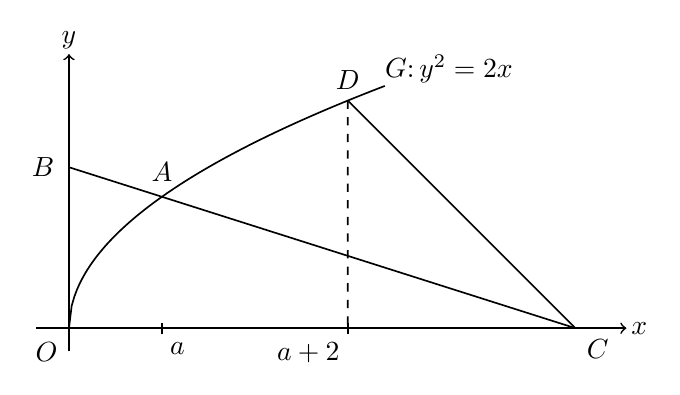
\begin{tikzpicture}[scale=1.18, semithick,
  every node/.style={inner sep=1.5pt}]
  % 坐标轴
  \draw[->] (-0.35,0) -- (6.0,0) node[anchor=west] {$x$};
  \draw[->] (0,-0.25) -- (0,2.95) node[anchor=south] {$y$};
  % 曲线 y=sqrt(2x)
  \draw plot[domain=0:3.4, samples=120] (\x, {sqrt(2*\x)});
  \node[anchor=south west] at (3.35,{sqrt(2*3.35)}) {$G\colon y^2=2x$};
  % 关键点
  \coordinate (O) at (0,0);
  \coordinate (A) at (1,1.4142136);
  \coordinate (B) at (0,1.7320508);
  \coordinate (C) at (5.45,0);
  \coordinate (D) at (3,2.4494897);
  % 直线 AB 延长到 C，D 处垂线与 CD
  \draw (B) -- (A) -- (C);
  \draw (D) -- (C);
  \draw[dashed] (D) -- (3,0);
  % x 轴上的位置刻度
  \draw (1,0.06) -- (1,-0.06);
  \draw (3,0.06) -- (3,-0.06);
  % 标注
  \node[anchor=north east] at ([xshift=-2pt,yshift=-3pt]O) {$O$};
  \node[anchor=south] at ([yshift=3pt]A) {$A$};
  \node[anchor=east] at ([xshift=-3pt]B) {$B$};
  \node[anchor=north west] at ([xshift=2pt,yshift=-2pt]C) {$C$};
  \node[anchor=south] at ([yshift=2pt]D) {$D$};
  \node[anchor=north west] at ([xshift=1pt,yshift=-3pt]1,0) {$a$};
  \node[anchor=north east] at ([xshift=-1pt,yshift=-3pt]3,0) {$a+2$};
\end{tikzpicture}
